% The Great Gatsby .tex
%-------------------------------------------------------------------------------
% Set Document
\documentclass[12pt,a4paper]{report}
%-------------------------------------------------------------------------------
% Packages
\usepackage{geometry}
\usepackage{graphicx}
\usepackage{amssymb}
\usepackage{float}
\usepackage{placeins}
%\renewcommand{\familydefault}{\sfdefault}
%-------------------------------------------------------------------------------
% Variables

%-------------------------------------------------------------------------------
% Fonts
%-------------------------------------------------------------------------------

% Document Head
\geometry{letterpaper}
\title{The Great Gatsby}
\author{F. Scott Fitzgerald}
\date{}
%-------------------------------------------------------------------------------
% Main Document
\begin{document}
\maketitle

\begin{figure}[ht!]
   \centering
     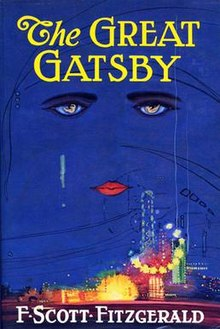
\includegraphics[width=0.25\textwidth]{images/jacket.jpg}
   \caption{The Great Gatsby}
\end{figure}

In my younger and more vulnerable years my father gave me some advice that I've been turning over in my mind ever since.

``Whenever you feel like criticising any one," he told me, ``just
remember that all the people in this world haven't had the advantages
that you've had." \cite{cite2}

\begin{figure}[h]
   \centering
     \includegraphics[width = 1 \textwidth]{example-image-a}
   \caption{The Great Gatsby}
\end{figure}

He didn't say any more but we've always been unusually communicative in a reserved way, and I understood that he meant a great deal more than that. In consequence I'm inclined to reserve all judgments, a habit that has opened upmany curious natures to me and also made me the victim of not a few veteranbores. The abnormal mind is quick to detect and attach itself to this qualitywhen it appears in a normal person, and so it came about that in college I wasunjustly accused of being a politician, because I was privy to the secret griefsof wild, unknown men. Most of the confidences were unsought--frequently I havefeigned sleep, preoccupation, or a hostile levity when I realized by someunmistakable sign that an intimate revelation was quivering on the horizon--forthe intimate revelations of young men or at least the terms in which theyexpress them are usually plagiaristic and marred by obvious suppressions.Reserving judgments is a matter of infinite hope. I am still a little afraid ofmissing something if I forget that, as my father snobbishly suggested, and Isnobbishly repeat, a sense of the fundamental decencies is parcelled outunequally at birth.

\FloatBarrier

And, after boasting this way of my tolerance, I come to the admissionthat it has a limit. Conduct may be founded on the hard rock or the wetmarshes but after a certain point I don't care what it's founded on.When I came back from the East last autumn I felt that I wanted theworld to be in uniform and at a sort of moral attention forever; Iwanted no more riotous excursions with privileged glimpses into thehuman heart. Only Gatsby, the man who gives his name to this book, wasexempt from my reaction--Gatsby who represented everything for which Ihave an unaffected scorn. If personality is an unbroken series ofsuccessful gestures, then there was something gorgeous about him, someheightened sensitivity to the promises of life, as if he were relatedto one of those intricate machines that register earthquakes tenthousand miles away. This responsiveness had nothing to do with thatflabby impressionability which is dignified under the name of the"creative temperament"--it was an extraordinary gift for hope, a romanticreadiness such as I have never found in any other person and which itis not likely I shall ever find again. No--Gatsby turned out all rightat the end; it is what preyed on Gatsby, what foul dust floated in thewake of his dreams that temporarily closed out my interest in theabortive sorrows and short-winded elations of men.

My family have been prominent, well-to-do people in this middle-westerncity for three generations. The Carraways are something of a clan and wehave a tradition that we're descended from the Dukes of Buccleuch, but theactual founder of my line was my grandfather's brother who came here infifty-one, sent a substitute to the Civil War and started the wholesalehardware business that my father carries on today.

I never saw this great-uncle but I'm supposed to look like him--withspecial reference to the rather hard-boiled painting that hangs inFather's office. I graduated from New Haven in 1915, just a quarter of acentury after my father, and a little later I participated in thatdelayed Teutonic migration known as the Great War. I enjoyed thecounter-raid so thoroughly that I came back restless. Instead of beingthe warm center of the world the middle-west now seemed like theragged edge of the universe--so I decided to go east and learn the bondbusiness. Everybody I knew was in the bond business so I supposed itcould support one more single man. All my aunts and uncles talked itover as if they were choosing a prep-school for me and finally said,"Why--ye-es" with very grave, hesitant faces. Father agreed to financeme for a year and after various delays I came east, permanently, Ithought, in the spring of twenty-two.

The practical thing was to find rooms in the city but it was a warmseason and I had just left a country of wide lawns and friendly trees,so when a young man at the office suggested that we take a housetogether in a commuting town it sounded like a great idea. He foundthe house, a weather beaten cardboard bungalow at eighty a month, butat the last minute the firm ordered him to Washington and I went outto the country alone. I had a dog, at least I had him for a few daysuntil he ran away, and an old Dodge and a Finnish woman who made my bedand cooked breakfast and muttered Finnish wisdom to herself over theelectric stove.
It was lonely for a day or so until one morning some man, more recentlyarrived than I, stopped me on the road.
"How do you get to West Egg village?" he asked helplessly.

I told him. And as I walked on I was lonely no longer. I was a guide, apathfinder, an original settler. He had casually conferred on me thefreedom of the neighborhood.

And so with the sunshine and the great bursts of leaves growing on thetrees--just as things grow in fast movies--I had that familiarconviction that life was beginning over again with the summer.

There was so much to read for one thing and so much fine health to bepulled down out of the young breath-giving air. I bought a dozenvolumes on banking and credit and investment securities and they stoodon my shelf in red and gold like new money from the mint, promising tounfold the shining secrets that only Midas and Morgan and Maecenasknew. And I had the high intention of reading many other books besides.I was rather literary in college--one year I wrote a series of verysolemn and obvious editorials for the "Yale News"--and now I was goingto bring back all such things into my life and become again that mostlimited of all specialists, the "well-rounded man." This isn't just anepigram--life is much more successfully looked at from a single window,after all.

It was a matter of chance that I should have rented a house in one ofthe strangest communities in North America. It was on that slenderriotous island which extends itself due east of New York and wherethere are, among other natural curiosities, two unusual formations ofland. Twenty miles from the city a pair of enormous eggs, identical incontour and separated only by a courtesy bay, jut out into the mostdomesticated body of salt water in the Western Hemisphere, the greatwet barnyard of Long Island Sound. They are not perfect ovals--like theegg in the Columbus story they are both crushed flat at the contactend--but their physical resemblance must be a source of perpetualconfusion to the gulls that fly overhead. To the wingless a morearresting phenomenon is their dissimilarity in every particular exceptshape and size.

I lived at West Egg, the--well, the less fashionable of the two, thoughthis is a most superficial tag to express the bizarre and not a littlesinister contrast between them. My house was at the very tip of theegg, only fifty yards from the Sound, and squeezed between two hugeplaces that rented for twelve or fifteen thousand a season. The one onmy right was a colossal affair by any standard--it was a factualimitation of some Hôtel de Ville in Normandy, with a tower on one side,spanking new under a thin beard of raw ivy, and a marble swimming pooland more than forty acres of lawn and garden. It was Gatsby's mansion.Or rather, as I didn't know Mr. Gatsby it was a mansion inhabited bya gentleman of that name. My own house was an eye-sore, but it was asmall eye-sore, and it had been overlooked, so I had a view of thewater, a partial view of my neighbor's lawn, and the consolingproximity of millionaires--all for eighty dollars a month.

Across the courtesy bay the white palaces of fashionable East Eggglittered along the water, and the history of the summer really beginson the evening I drove over there to have dinner with the TomBuchanans. Daisy was my second cousin once removed and I'd known Tomin college. And just after the war I spent two days with them inChicago.
Her husband, among various physical accomplishments, had been one ofthe most powerful ends that ever played football at New Haven--anational figure in a way, one of those men who reach such an acutelimited excellence at twenty-one that everything afterward savors ofanti-climax. His family were enormously wealthy--even in college hisfreedom with money was a matter for reproach--but now he'd left Chicagoand come east in a fashion that rather took your breath away: forinstance he'd brought down a string of polo ponies from Lake Forest.It was hard to realize that a man in my own generation was wealthyenough to do that.
Why they came east I don't know. They had spent a year in France, for noparticular reason, and then drifted here and there unrestfully whereverpeople played polo and were rich together. This was a permanent move,said Daisy over the telephone, but I didn't believe it--I had no sightinto Daisy's heart but I felt that Tom would drift on forever seekinga little wistfully for the dramatic turbulence of some irrecoverablefootball game.

And so it happened that on a warm windy evening I drove over to EastEgg to see two old friends whom I scarcely knew at all. Their house waseven more elaborate than I expected, a cheerful red and white GeorgianColonial mansion overlooking the bay. The lawn started at the beachand ran toward the front door for a quarter of a mile, jumping oversun-dials and brick walks and burning gardens--finally when it reachedthe house drifting up the side in bright vines as though from themomentum of its run. The front was broken by a line of French windows,glowing now with reflected gold, and wide open to the warm windyafternoon, and Tom Buchanan in riding clothes was standing with hislegs apart on the front porch.

He had changed since his New Haven years. Now he was a sturdy, straw hairedman of thirty with a rather hard mouth and a supercilious manner.Two shining, arrogant eyes had established dominance over his face andgave him the appearance of always leaning aggressively forward. Noteven the effeminate swank of his riding clothes could hide the enormouspower of that body--he seemed to fill those glistening boots until hestrained the top lacing and you could see a great pack of muscleshifting when his shoulder moved under his thin coat. It was a bodycapable of enormous leverage--a cruel body.

His speaking voice, a gruff husky tenor, added to the impression offractiousness he conveyed. There was a touch of paternal contempt init, even toward people he liked--and there were men at New Haven who hadhated his guts.

"Now, don't think my opinion on these matters is final," he seemed tosay, "just because I'm stronger and more of a man than you are." Wewere in the same Senior Society, and while we were never intimate Ialways had the impression that he approved of me and wanted me to likehim with some harsh, defiant wistfulness of his own.
We talked for a few minutes on the sunny porch.

"I've got a nice place here," he said, his eyes flashing aboutrestlessly.


\bibliographystyle{abbrv}
\bibliography{bibliography/TheGreatGatsby}
\end{document}
